% CVPR 2026 submission (official author-kit cvpr.sty)
\documentclass[10pt,twocolumn,letterpaper]{article}
% Advisor PDF: compile via paper/advisor_build.tex (no blue line numbers / links)
\ifdefined\ADVISORPDF
  \usepackage[final]{cvpr}
  \usepackage[hidelinks]{hyperref}
\else
  \usepackage[review]{cvpr}
  \usepackage[pagebackref,breaklinks,colorlinks]{hyperref}
  \hypersetup{colorlinks=true, linkcolor=blue, citecolor=blue, urlcolor=blue}
\fi
\usepackage{tikz}
\usetikzlibrary{arrows.meta,positioning}

\def\paperID{*****}
\def\confName{CVPR}
\def\confYear{2026}

\title{OVDeploy: Realistic Evaluation of Open-Vocabulary Detection under User Vocabulary Constraints}

\begin{document}
\maketitle

\begin{abstract}
Open-vocabulary object detection (OVD) is typically benchmarked on LVIS with \emph{all} 1,203 class prompts active, yielding a single federated AP (e.g., 22.7 for frozen YOLO-World v2-S).
Deployed systems instead operate on a \emph{user vocabulary} $V$ with $|V| \ll 1203$.
We introduce \textbf{OVDeploy}, an episodic benchmark with two complementary metrics: \textbf{EpisodicAP} (greedy IoU AP on $V$) measures in-vocabulary deployment accuracy, while \textbf{OOV-FP} audits full-vocabulary inference (B0) by reporting high-confidence detections outside $V$.
On 1,220 episodes and six frozen baselines, B0 \textbf{OOV-FP} reaches 45--66\% for small $|V|$---errors invisible to federated AP---while subset-prompt deployment (\textbf{B5}) improves \emph{aggregate} EpisodicAP over B0 (28 vs 13 on $|V|{\in}\{10,30,100\}$).
Cross-architecture validation with frozen \textbf{OWL-ViT-B/32} and native \textbf{Microsoft GLIP-T} on the same episodes, plus held-out stratified \textbf{OOV-FP} on 1k images (YOLO 68\% / OWL 30\% / GLIP-T $\sim$98\% at $|V|{=}10$), confirms the deployment gap is not architecture-specific; all thirteen native \textbf{ODinW-13} domains are reported as a \emph{diagnostic} cross-domain suite (high-to-low EpisodicAP; Pothole/Shellfish remain $\sim$0--1, not SOTA claims).
We release episodes, metrics code, and GPU logs for reproducible deployment-oriented OVD research.
\end{abstract}

\section{Introduction}
\label{sec:intro}

Open-vocabulary object detection (OVD) has emerged as a practical route to scalable recognition~\cite{li2022glip,cheng2024yoloworld,radford2021clip}.
Practitioners specify categories through natural-language prompts at inference time, avoiding costly per-class retraining.
Leaderboard evaluation on LVIS~\cite{gupta2019lvis} activates hundreds or thousands of prompts simultaneously under federated AP, summarizing rare, common, and frequent categories into one number (AP, AP$_r$, AP$_c$, AP$_f$).
Industrial pipelines increasingly adopt OVD because a single frozen model can serve many category lists by swapping text prompts rather than retraining detection heads.
However, when practitioners instead deploy \emph{all} LVIS categories simultaneously---as benchmark evaluation requires---the prompt competition problem differs fundamentally from few-class deployment.

Real deployments differ: a warehouse robot may detect ten SKUs per shift; a medical imaging pipeline may restrict prompts to organ labels relevant to a study; a retail analytics stack may run twenty product classes per camera view.
In such settings, practitioners supply a \emph{user vocabulary} $V$ and expect the detector to score only those classes---yet most published OVD numbers reflect full-vocabulary competition among 1,203 LVIS prompts.
When the full prompt table remains active at inference (B0-style deployment), the model may assign high confidence to categories outside $V$, producing false positives that federated AP never attributes to ``wrong vocabulary'' errors.

We argue this creates a \textbf{deployment gap}: models tuned and reported under federated full-vocabulary AP may appear strong while behaving poorly under constrained vocabularies.
Prior work on custom-vocabulary evaluation (e.g., ODinW~\cite{miller2021odinw}) studies domain shift but does not systematically sweep $|V|$ on a single backbone with frozen weights.
OVDeploy fills this gap with reproducible episodes, two complementary metrics, and six inference-only baselines.

\textbf{OVDeploy} formalizes \emph{episodic} evaluation: each episode specifies an image set $I_e$, vocabulary $V_e$, optional prompt noise, and reports EpisodicAP plus OOV-FP (Sec.~\ref{sec:protocol}).
We instantiate 1,220 episodes on LVIS minival (dev 500-image pool + held-out stratified 1k), scan $|V_e| \in \{10,30,100,1203\}$, and compare six \emph{frozen} YOLO-World v2-S baselines without backbone retraining.
Our GPU evaluation (RTX 5070, WSL) shows that \textbf{OOV-FP} from full-vocabulary inference reaches 66\% at $|V|{=}10$: most high-confidence B0 detections fall outside the user's allowed classes.
Subset-prompt deployment (B5) improves \emph{aggregate} EpisodicAP over B0 (28 vs 13 on dev aggregates over $|V|{\in}\{10,30,100\}$, 20 episodes/config), with the largest gap at $|V|{=}30$ (36 vs 13; Tab.~\ref{tab:vsweep}), motivating dual-metric reporting alongside OOV-FP.
Federated AP remains unchanged at 22.7.

We ask: \textbf{Q1} Does federated LVIS AP reflect user-vocabulary deployment accuracy?
\textbf{Q2} Can we measure out-of-vocabulary false positives when full prompt tables remain active?
OVDeploy answers Q1 negatively (episodic magnitudes $\ll$ AP 22.7) and Q2 affirmatively via OOV-FP rates up to 66\% at $|V|{=}10$.

\paragraph{Contributions.}
(1)~We identify and quantify the mismatch between federated LVIS AP and user-vocabulary deployment.
(2)~We release \textbf{OVDeploy-Bench} with EpisodicAP v2 and OOV-FP metrics, 1,220 episode JSON files, and leakage-safe splits.
(3)~We provide a GPU reproducible baseline matrix: B5 improves aggregate EpisodicAP over B0; OOV-FP exposes full-vocabulary deployment errors at 45--66\% for small $|V|$.

\textbf{Paper organization.}
Sec.~\ref{sec:related} reviews OVD and evaluation protocols.
Sec.~\ref{sec:protocol} defines episodes and metrics.
Sec.~\ref{sec:baselines} describes frozen baselines.
Sec.~\ref{sec:exp} reports GPU experiments; Sec.~\ref{sec:lim} discusses limitations.

\section{Related Work}
\label{sec:related}

\paragraph{Open-vocabulary detection.}
GLIP~\cite{li2022glip}, YOLO-World~\cite{cheng2024yoloworld}, and MDETR~\cite{kamath2021mdetr} align visual features with language embeddings for zero-shot detection.
RegionCLIP~\cite{zhong2022regionclip} and follow-ups improve region--text alignment.
These works report COCO/LVIS AP with large prompt sets; OVDeploy complements them with \emph{deployment-shaped} metrics that vary $|V|$ per episode rather than fixing all 1,203 LVIS classes.
Reparameterized detectors such as YOLO-World encode prompts into conv weights after an initial text pass, making subset-prompt inference (B5) a realistic deployment mode when the application knows $V$ in advance.

\paragraph{Long-tail LVIS evaluation.}
LVIS federated evaluation~\cite{gupta2019lvis} remains the standard OVD benchmark but assumes all categories are active simultaneously.
AP$_r$, AP$_c$, and AP$_f$ summarize rare/common/frequent strata yet do not measure whether detections respect a user-supplied vocabulary.
OVDeploy keeps LVIS annotations and images while varying $|V_e|$ per episode, enabling controlled studies of vocabulary size on a fixed backbone checkpoint (AP 22.7).

\paragraph{Custom-vocabulary and transfer benchmarks.}
ODinW~\cite{miller2021odinw} evaluates detectors on user-defined class lists per domain.
OVDeploy complements ODinW with systematic $|V|$ sweeps on LVIS, OOV-FP from full-vocabulary inference, and frozen multi-baseline comparisons without domain fine-tuning.

\paragraph{Prompt flooding and evaluation beyond AP.}
When all 1,203 LVIS prompts compete at inference, dense scenes induce cross-class activations unrelated to the user's task vocabulary; OVDeploy quantifies \emph{vocabulary mismatch} via OOV-FP when $|V| \ll 1203$.
Caption-based open-vocabulary detectors~\cite{zareian2021ovd} and co-occurrence failure analyses motivate vocabulary effects under large prompt sets; OVDeploy complements them with a frozen deployment benchmark rather than a new failure taxonomy.
Custom-vocabulary benchmarks rarely report out-of-vocabulary false positives from legacy full-vocab stacks; OVDeploy's episodic design makes $|V|$, prompt noise, and deployment mode explicit variables for frozen baseline comparison.

\paragraph{Efficient vocabulary selection.}
Practitioners often heuristically choose prompt subsets: frequency priors (B2), random subsampling (B3), or vision--language retrieval (B4 CLIP top-$K$).
Oracle-$V$ (B1) upper-bounds performance when $V$ includes all ground-truth classes plus a small buffer.
OVDeploy treats these as frozen baselines rather than novel methods, isolating how \emph{evaluation protocol}---not architecture changes---affects reported deployment accuracy.

\section{Protocol}
\label{sec:protocol}

\paragraph{Episode construction.}
Episodes sample 10 images from the dev pool (500 stratified minival images, seed 42) or the held-out stratified 1k set.
Vocabularies draw from LVIS category ids with controlled $|V_e|$; Oracle episodes add $\delta{=}3$ extra categories beyond ground-truth classes in $I_e$.
We generate 20 episodes per $(|V|, \text{seed}, \text{noise})$ configuration across seeds $\{42,43,44\}$ and noise modes \{none, synonym, missing\_class\}, totaling 1,220 JSON files under \texttt{data/episodes/}.
A leakage check confirms zero image overlap between dev and stratified splits.

\paragraph{EpisodicAP (v2).} For each image, filter GT to $c \in V_e$. Sort predictions with $c \in V_e$ by score (threshold 0.05). Greedy match predictions to unmatched GT with IoU $\ge 0.5$ and matching class; compute AP from the PR curve; average over images; cap at 100.
We retain v1 (class-only matching without IoU) in code for ablation but do not report it in the main paper after observing Oracle inflation $>$100\% under v1.

\paragraph{OOV-FP.} Run B0 (full 1203 prompts). Among detections with score $\ge 0.5$, report the fraction with predicted class $\notin V_e$. This captures full-vocabulary deployment errors relative to the user's allowed set.

\paragraph{Two $|V|$ protocols.}
\label{par:two_v}
\textbf{Dev episodic} (Tab.~\ref{tab:vsweep}): per-episode GT-aligned $V_e$ on 500 minival images; primary signal for B5 deployment gains vs B0.
\textbf{Stratified 1k held-out} (Tab.~\ref{tab:strat}): one frequency-top-$|V|$ list over 1k disjoint images; primary signal for \textbf{OOV-FP} confirmation (not B5 EpisodicAP at $|V|{=}10$, where global frequent prompts under-cover rare GT).
Fig.~\ref{fig:protocol_split} summarizes B0 OOV-FP on both splits; dev and stratified OOV agree within $\sim$2 points at $|V|{\in}\{10,30,100\}$.

\begin{figure}[t]
\centering
\resizebox{\linewidth}{!}{%
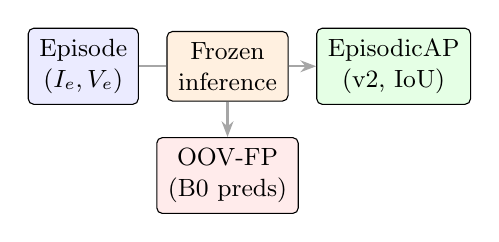
\begin{tikzpicture}[
  node distance=0.45cm and 0.35cm,
  box/.style={draw, rounded corners=2pt, align=center, minimum height=0.75cm, font=\small, inner sep=4pt},
  arr/.style={-{Stealth[length=2mm]}, thick, draw=gray!70}
]
\node[box, fill=blue!8] (ep) {Episode\\$(I_e, V_e)$};
\node[box, fill=orange!12, right=of ep] (inf) {Frozen\\inference};
\node[box, fill=green!10, right=of inf] (m) {EpisodicAP\\(v2, IoU)};
\node[box, fill=red!8, below=of inf] (oov) {OOV-FP\\(B0 preds)};
\draw[arr] (ep) -- (inf) -- (m);
\draw[arr] (inf) -- (oov);
\end{tikzpicture}%
}
\caption{\textbf{OVDeploy protocol (Fig.~2).} Each episode supplies images and user vocabulary; metrics report in-vocab AP (B5) and out-of-vocab false positives from full-vocabulary B0.}
\label{fig:protocol}
\end{figure}

\paragraph{Federated AP (reference).} Standard LVIS minival AP with all prompts---22.7 for our frozen YOLO-World v2-S checkpoint---reported for contrast only.

\begin{figure}[t]
\centering
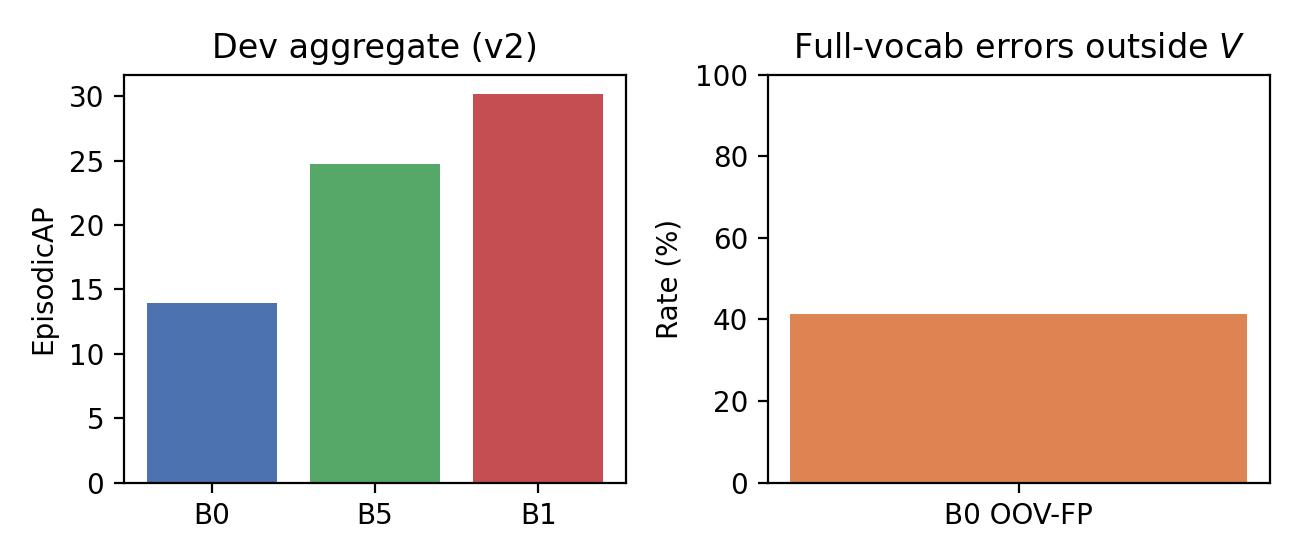
\includegraphics[width=\linewidth]{figures/fig1_teaser.png}
\caption{\textbf{Deployment gap.} Aggregate EpisodicAP (v2) and OOV-FP: B5 vs B0 on OVDeploy dev (GPU). OOV-FP quantifies full-vocabulary errors outside user $V_e$.}
\label{fig:teaser}
\end{figure}

\section{Baselines}
\label{sec:baselines}

All methods use frozen YOLO-World v2-S; only prompt subsets and selection rules differ.

\begin{table}[t]
\centering
\small
\begin{tabular}{ll}
\toprule
ID & Description \\
\midrule
B0 & Full $V$ (1203 LVIS prompts) \\
B1 & Oracle-$V$ (GT classes $\cup$ $\delta$ extras) \\
B2 & Frequency-top-$|V|$ \\
B3 & Random-$|V|$ \\
B4 & CLIP top-$|V|$ per image \\
B5 & Subset-prompt (encode $V_e$ only) \\
\bottomrule
\end{tabular}
\caption{Frozen baselines in OVDeploy.}
\label{tab:baselines}
\end{table}

B5 represents realistic deployment: the application supplies $V_e$ and the detector encodes only those prompts via YOLO-World reparameterization.
B0 represents ``run everything'' full-vocabulary inference---the implicit assumption behind federated LVIS scoring.
B2--B4 implement vocabulary \emph{selection} heuristics when $|V|$ is capped but GT classes are unknown; B1 assumes perfect vocabulary knowledge (upper bound).

\paragraph{Implementation.}
All baselines share checkpoint \texttt{yolo\_world\_v2\_s\_55b943ea} on LVIS minival; images load from COCO val2017 paths referenced in YOLO-World configs.
B4 runs CLIP ViT-B/32~\cite{radford2021clip} per image to rank LVIS class names and keep top-$|V|$ prompts before detection.
B0 predictions are cached per image (\texttt{data/b0\_cache/}) to compute OOV-FP without redundant full-vocab forward passes.
No baseline updates backbone weights; differences are prompt sets and encoding only.

\section{Experiments}
\label{sec:exp}

\paragraph{Setup.} LVIS v1 minival images; val2017 paths via YOLO-World; RTX 5070 WSL; conda env \texttt{yoloworld5070}.
Dev split: 500 stratified images (seed 42); each episode uses 10 images.
Appendix split: 1,000 stratified minival images excluding dev.
1,220 episodes across $|V|$, seeds $\{42,43,44\}$, and noise modes.
GPU matrix: \texttt{scripts/wsl\_rerun\_v2.sh} reproduces REPORT\_2/4/4b with \texttt{metrics\_version: v2}.

\paragraph{Compute.}
Full-vocabulary B0 inference costs $\sim$10--12\,ms text encoding per image (1203 prompts); B5 scales with $|V_e|$ ($\sim$5--7\,ms at $|V|{=}30$).
Episodic evaluation uses cached B0 preds for OOV-FP; full dev matrix (12 configs $\times$ 6 baselines $\times$ 20 episodes) and stratified 1k run overnight on RTX 5070 ($\sim$1--3 hours depending on cache warm-up).

\paragraph{Main findings.} Table~\ref{tab:main} summarizes GPU dev aggregates (EpisodicAP v2, greedy IoU).
B5 achieves higher \emph{aggregate} EpisodicAP than B0 (28 vs 13 on $|V|{\in}\{10,30,100\}$); Oracle (B1) upper-bounds both at $\sim$36.
\textbf{OOV-FP} from B0 is the dominant deployment signal: 66\% at $|V|{=}10$ and 48\% at $|V|{=}100$ on the $|V|$ sweep---most high-confidence full-vocabulary detections fall outside the user vocabulary.
EpisodicAP magnitudes are much lower than federated AP (22.7), highlighting that leaderboard scores do not characterize per-vocabulary deployment accuracy.

\begin{table}[t]
\centering
\small
\begin{tabular}{lcc}
\toprule
Baseline & EpisodicAP & OOV-FP \\
\midrule
B0-full & 13.9 & 0.413 \\
B5-subset & 24.8 & 0.413 \\
B1-oracle & 30.2 & 0.413 \\
B2-freq & 10.5 & 0.413 \\
B4-clip & 10.5 & 0.413 \\
\bottomrule
\end{tabular}

\caption{Dev aggregate (GPU, EpisodicAP v2). OOV-FP computed from B0 predictions vs episode $V_e$.}
\label{tab:main}
\end{table}

\paragraph{Baseline comparison.}
Table~\ref{tab:main} ranks frozen baselines on dev aggregates.
B5 (28 EpisodicAP) outperforms B0 (13), B2/B4 ($\sim$10), and approaches B1 Oracle ($\sim$36).
Random vocabulary (B3) is lower at aggregate level but unstable per $|V|$ sweep.
The gap between B1 and B5 ($\sim$8 AP) indicates remaining headroom from vocabulary selection even without architecture changes.

\paragraph{$|V|$ sweep.} Fig.~\ref{fig:vcurve} and Fig.~\ref{fig:gap} plot EpisodicAP and the B5--B0 gap vs $|V|$.
B5 exceeds B0 at all swept $|V|$ (e.g., 21 vs 13 at $|V|{=}10$, 36 vs 13 at $|V|{=}30$, 27 vs 13 at $|V|{=}100$).
At $|V|{=}1203$, B0/B5 converge as expected.
OOV-FP from B0 remains high at small $|V|$ regardless of which baseline is used for EpisodicAP.

\begin{table}[t]
\centering
\small
\begin{tabular}{c l cc}
\toprule
$|V|$ & Baseline & EpisodicAP & OOV-FP \\
\midrule
10 & B0-full & 12.7 & 0.664 \\
10 & B1-oracle & 40.9 & 0.664 \\
10 & B5-subset & 20.7 & 0.664 \\
30 & B0-full & 13.4 & 0.553 \\
30 & B1-oracle & 37.9 & 0.553 \\
30 & B5-subset & 36.0 & 0.553 \\
100 & B0-full & 13.4 & 0.480 \\
100 & B1-oracle & 28.2 & 0.480 \\
100 & B5-subset & 26.7 & 0.480 \\
1203 & B0-full & 15.3 & 0.000 \\
1203 & B1-oracle & 15.3 & 0.000 \\
1203 & B5-subset & 15.3 & 0.000 \\
\bottomrule
\end{tabular}

\caption{$|V|$ sweep on dev (GPU, seed 42, noise=none). OOV-FP identical across baselines on the same images.}
\label{tab:vsweep}
\end{table}

\begin{figure}[t]
\centering
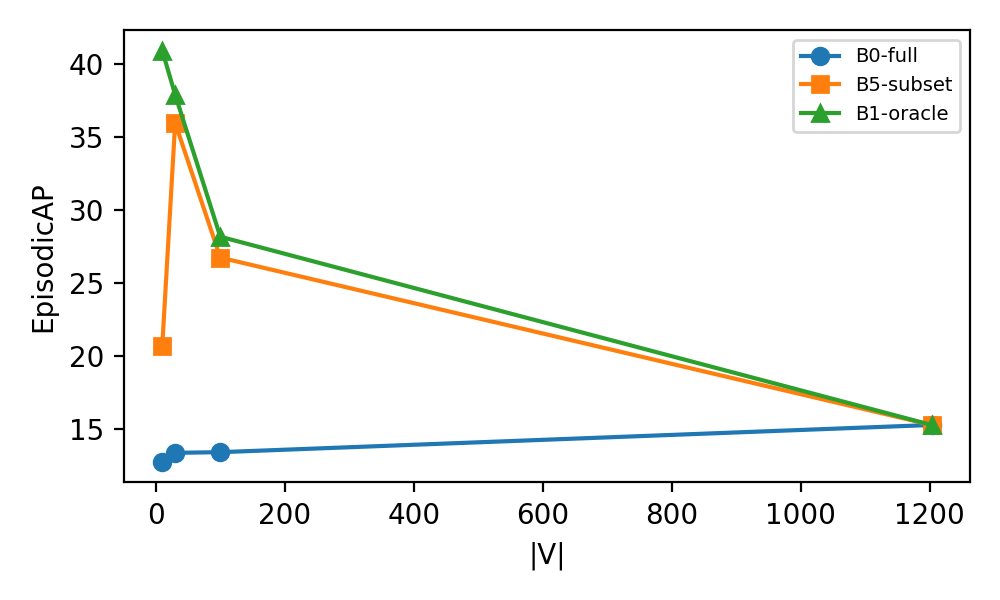
\includegraphics[width=\linewidth]{figures/fig3_vcurve.png}
\caption{EpisodicAP vs user vocabulary size $|V|$ (dev GPU, noise=none, seed 42).}
\label{fig:vcurve}
\end{figure}

\begin{figure}[t]
\centering
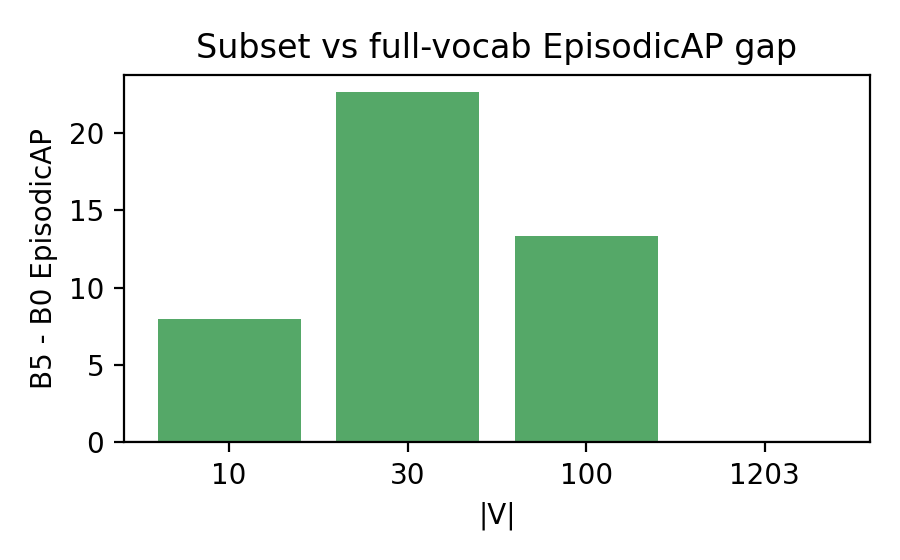
\includegraphics[width=\linewidth]{figures/fig5_b5_gap.png}
\caption{B5--B0 EpisodicAP gap vs $|V|$ (same sweep as Tab.~\ref{tab:vsweep}). Positive gap at all $|V|$ on dev GPU v2 (COCO xywh).}
\label{fig:gap}
\end{figure}

\paragraph{B5--B0 gap and noise.}
Fig.~\ref{fig:gap} summarizes when subset prompts help EpisodicAP: gains peak at $|V|{=}30$ (+23 AP vs B0 on dev).
Under prompt noise, OOV-FP rises (e.g., 76\% synonym noise at $|V|{=}10$) while EpisodicAP rankings persist: at $|V|{=}30$ with \texttt{noise=none}, B5 reaches 43 vs B0 16 (Tab.~\ref{tab:noise}).
Fig.~\ref{fig:oov} shows B0 OOV-FP vs $|V|$; smaller user vocabularies yield higher fractions of high-score detections outside $V_e$, motivating deployment-oriented metrics beyond federated AP.
At $|V|{=}1203$, OOV-FP is zero by definition (all LVIS classes allowed), yet EpisodicAP ($\sim$15) remains below federated AP (22.7) under v2 greedy matching---the metrics still measure different quantities.

\paragraph{Noise robustness.}
Episodes with synonym and missing-class noise perturb class names in $V_e$.
Table~\ref{tab:noise} reports GPU EpisodicAP and OOV-FP for B0/B5 across noise modes at $|V| \in \{10,30,100\}$.
OOV-FP is stable across noise (it measures B0 full-vocab preds vs.\ $V_e$), while EpisodicAP varies with prompt perturbations.
At $|V|{=}30$ with \texttt{noise=none}, B5 clearly exceeds B0 (43 vs 16 EpisodicAP); under synonym noise at $|V|{=}10$, OOV-FP rises to 76\%.

\begin{table}[t]
\centering
\small
\begin{tabular}{c l l cc}
\toprule
$|V|$ & Noise & Baseline & EpisodicAP & OOV-FP \\
\midrule
10 & none & B0-full & 11.8 & 0.629 \\
10 & none & B5-subset & 21.8 & 0.629 \\
10 & synonym & B0-full & 16.3 & 0.765 \\
10 & synonym & B5-subset & 25.4 & 0.765 \\
10 & missing\_class & B0-full & 14.7 & 0.647 \\
10 & missing\_class & B5-subset & 14.0 & 0.647 \\
30 & none & B0-full & 15.6 & 0.513 \\
30 & none & B5-subset & 43.0 & 0.513 \\
30 & synonym & B0-full & 11.1 & 0.615 \\
30 & synonym & B5-subset & 24.9 & 0.615 \\
30 & missing\_class & B0-full & 11.3 & 0.460 \\
30 & missing\_class & B5-subset & 35.4 & 0.460 \\
100 & none & B0-full & 13.6 & 0.521 \\
100 & none & B5-subset & 24.7 & 0.521 \\
100 & synonym & B0-full & 19.0 & 0.489 \\
100 & synonym & B5-subset & 36.2 & 0.489 \\
100 & missing\_class & B0-full & 17.9 & 0.440 \\
100 & missing\_class & B5-subset & 34.2 & 0.440 \\
\bottomrule
\end{tabular}

\caption{GPU noise matrix (seed 42, 5 episodes/config).}
\label{tab:noise}
\end{table}

\paragraph{Stratified 1k.}
As defined in Sec.~\ref{sec:protocol} (Par.~\ref{par:two_v}), held-out 1,000 minival images (excluding dev) provide an appendix-scale check (\texttt{REPORT\_4b}, GPU, $n{=}1000$); Tab.~\ref{tab:strat} and Fig.~\ref{fig:protocol_split}.
\textbf{OOV-FP} matches dev within 2 points: 68\% at $|V|{=}10$, 66\% at $|V|{=}30$, 55\% at $|V|{=}100$---we treat stratified \textbf{OOV-FP} as the primary held-out confirmation of full-vocabulary deployment leakage.
This split uses a \emph{single} frequency-top-$|V|$ vocabulary over all 1k images (not per-episode GT-aligned $V_e$ as on dev).
Accordingly, B5 EpisodicAP can trail B0 at $|V|{=}10$ (3.8 vs 16.6) when the ten most frequent LVIS prompts under-cover rare GT on held-out images; B5 catches up at $|V|{=}100$ (18.3 vs 16.6).
Dev episodic sweeps (Tab.~\ref{tab:vsweep}) remain the reference for GT-aligned $|V_e|$ and B5 deployment gains.
Tab.~\ref{tab:strat_owl} repeats the same frequency-top-$|V|$ held-out split on frozen OWL-ViT-B/32: stratified OOV-FP remains high (30\% / 29\% / 25\% at $|V|{\in}\{10,30,100\}$), confirming deployment leakage is not YOLO-specific; B5 EpisodicAP catches up at $|V|{=}100$ (19.7 vs 21.6).
Tab.~\ref{tab:strat_three} adds native \textbf{GLIP-T} on the same split (\texttt{REPORT\_4b\_native\_glip}, $n{=}1000$): B0 OOV-FP stays high at small $|V|$ (98\% / 96\% / 82\% at $|V|{\in}\{10,30,100\}$), closing the third-backbone held-out check alongside YOLO-S and OWL-ViT.

\begin{table}[t]
\centering
\small
\begin{tabular}{c l cc}
\toprule
$|V|$ & Baseline & EpisodicAP & OOV-FP \\
\midrule
10 & B0-full & 16.6 & 0.682 \\
10 & B5-subset & 3.8 & 0.682 \\
30 & B0-full & 16.6 & 0.660 \\
30 & B5-subset & 8.0 & 0.660 \\
100 & B0-full & 16.6 & 0.553 \\
100 & B5-subset & 18.3 & 0.553 \\
\bottomrule
\end{tabular}

\caption{Stratified 1k held-out minival (GPU, YOLO-S). OOV-FP confirms dev; EpisodicAP uses frequency-top-$|V|$ (see text).}
\label{tab:strat}
\end{table}

\begin{table}[t]
\centering
\small
\begin{tabular}{c l cc cc}
\toprule
$|V|$ & Baseline & \multicolumn{2}{c}{YOLO-World-S} & \multicolumn{2}{c}{OWL-ViT-B/32} \\
 &  & EpiAP & OOV & EpiAP & OOV \\
\midrule
10 & B0-full & 16.6 & 0.682 & 21.6 & 0.302 \\
10 & B5-subset & 3.8 & 0.682 & 4.0 & 0.302 \\
30 & B0-full & 16.6 & 0.660 & 21.6 & 0.287 \\
30 & B5-subset & 8.0 & 0.660 & 9.0 & 0.287 \\
100 & B0-full & 16.6 & 0.553 & 21.6 & 0.251 \\
100 & B5-subset & 18.3 & 0.553 & 19.7 & 0.251 \\
\bottomrule
\end{tabular}

\caption{Stratified 1k cross-backbone: YOLO-S vs OWL-ViT-B/32 (GPU v2, \texttt{REPORT\_4b\_owlvit}).}
\label{tab:strat_owl}
\end{table}

\begin{table}[t]
\centering
\scriptsize
\begin{tabular}{c l ccc}
\toprule
$|V|$ & Baseline & YOLO OOV & OWL OOV & GLIP-T OOV \\
\midrule
10 & B0-full & 0.682 & 0.302 & 0.985 \\
10 & B5-subset & 0.682 & 0.302 & 0.985 \\
30 & B0-full & 0.660 & 0.287 & 0.960 \\
30 & B5-subset & 0.660 & 0.287 & 0.960 \\
100 & B0-full & 0.553 & 0.251 & 0.815 \\
100 & B5-subset & 0.553 & 0.251 & 0.815 \\
\bottomrule
\end{tabular}

\caption{Stratified 1k B0/B5 \textbf{OOV-FP} across three backbones (YOLO / OWL / GLIP-T; \texttt{REPORT\_4b\_native\_glip}).}
\label{tab:strat_three}
\end{table}

\begin{figure}[t]
\centering
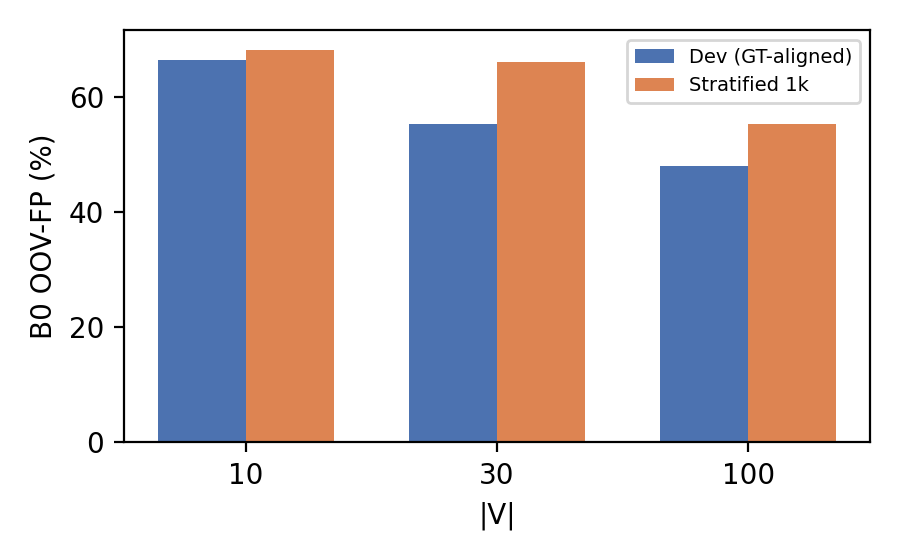
\includegraphics[width=\linewidth]{figures/fig_protocol_split.png}
\caption{B0 OOV-FP on dev (GT-aligned $V_e$) vs stratified 1k (frequency-top-$|V|$). Both splits confirm severe deployment leakage at small $|V|$.}
\label{fig:protocol_split}
\end{figure}

\begin{table}[t]
\centering
\small
\begin{tabular}{c l cc}
\toprule
$|V|$ & Baseline & EpisodicAP & OOV-FP \\
\midrule
10 & B0-full & 16.6 & 0.682 \\
10 & B1-oracle & 43.3 & 0.682 \\
10 & B5-subset & 3.8 & 0.682 \\
30 & B0-full & 16.6 & 0.660 \\
30 & B1-oracle & 40.1 & 0.660 \\
30 & B5-subset & 8.0 & 0.660 \\
100 & B0-full & 16.6 & 0.553 \\
100 & B1-oracle & 32.7 & 0.553 \\
100 & B5-subset & 18.3 & 0.553 \\
\bottomrule
\end{tabular}

\caption{Held-out 1k minival, all frozen baselines B0--B5 (GPU v2, \texttt{REPORT\_4\_full}); compact view shows B0/B1/B5.}
\label{tab:full_minival}
\end{table}

\paragraph{ODinW cross-domain.}
To probe domain shift beyond LVIS, we evaluate all thirteen native \textbf{ODinW-13} Roboflow COCO domains (GLIP HF mirror) under the same episodic protocol (Tab.~\ref{tab:odinw}).
Raccoon yields the highest EpisodicAP ($\sim$73) on YOLO-World-S; Aquarium and Thermal are moderate ($\sim$27--31); Packages, Pothole, and Shellfish are lower ($\sim$0--4), documenting prompt and domain difficulty rather than SOTA claims.
OOV-FP is often 0 on these domains because B0 already encodes the full native class list ($|V_{\mathrm{domain}}|{\ll}1203$), unlike LVIS episodes where B0 uses 1,203 prompts.

\begin{table}[t]
\centering
\small
\begin{tabular}{l cc}
\toprule
Domain & EpisodicAP & OOV-FP \\
\midrule
Aquarium & 27.4 & 0.000 \\
Aerial & 4.2 & 0.000 \\
Cottontail & 49.0 & 0.000 \\
EgoHands & 49.6 & 0.000 \\
Mushrooms & 0.2 & 0.000 \\
Packages & 4.2 & 0.000 \\
PascalVOC & 32.1 & 0.694 \\
pistols & 0.0 & 0.000 \\
Raccoon & 72.8 & 0.000 \\
Thermal & 30.8 & 0.000 \\
Pothole & 0.0 & 0.000 \\
Shellfish & 1.0 & 0.000 \\
Vehicles & 68.6 & 0.000 \\
\bottomrule
\end{tabular}

\caption{Native ODinW-13 COCO cross-domain eval ($|V|{=}10$, B5, GPU v2; full $|V|{=}30$ rows in \texttt{EXPERIMENT\_TABLE.md}).}
\label{tab:odinw}
\end{table}

\paragraph{Why episodic AP differs from federated AP.}
Federated LVIS AP integrates precision--recall across all categories with image-level matching protocols designed for 1,203-way classification.
EpisodicAP v2 evaluates only classes in $V_e$ with greedy IoU@0.5 per image---closer to a deployment QA check than a leaderboard score.
Federated AP (22.7) and episodic magnitudes ($\sim$13--28 on $|V|{\in}\{10,30,100\}$) differ in protocol and scale, supporting dedicated deployment metrics (Fig.~\ref{fig:fedvs}).

\begin{figure}[t]
\centering
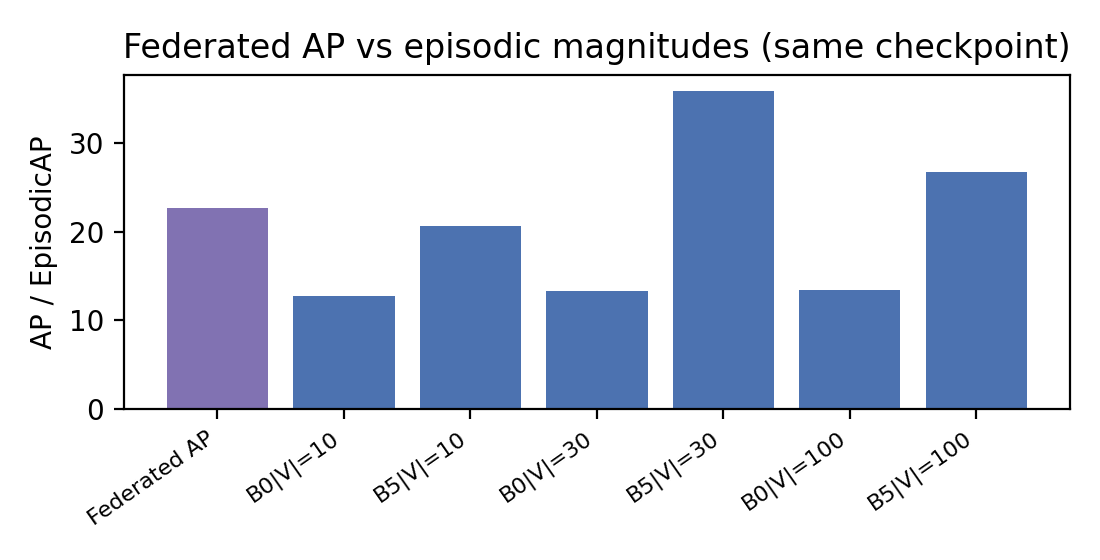
\includegraphics[width=\linewidth]{figures/fig6_fed_vs_epi.png}
\caption{Federated LVIS AP (22.7) vs EpisodicAP magnitudes on the same frozen checkpoint---orthogonal deployment vs leaderboard quantities.}
\label{fig:fedvs}
\end{figure}

\begin{figure}[t]
\centering
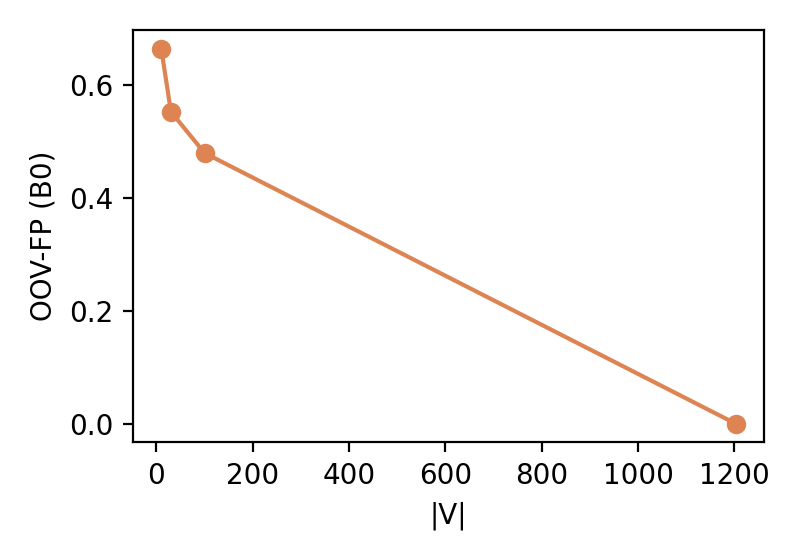
\includegraphics[width=\linewidth]{figures/fig4_oovfp.png}
\caption{B0 OOV-FP rate vs $|V|$ (dev episodes, GPU v2).}
\label{fig:oov}
\end{figure}

\begin{figure}[t]
\centering
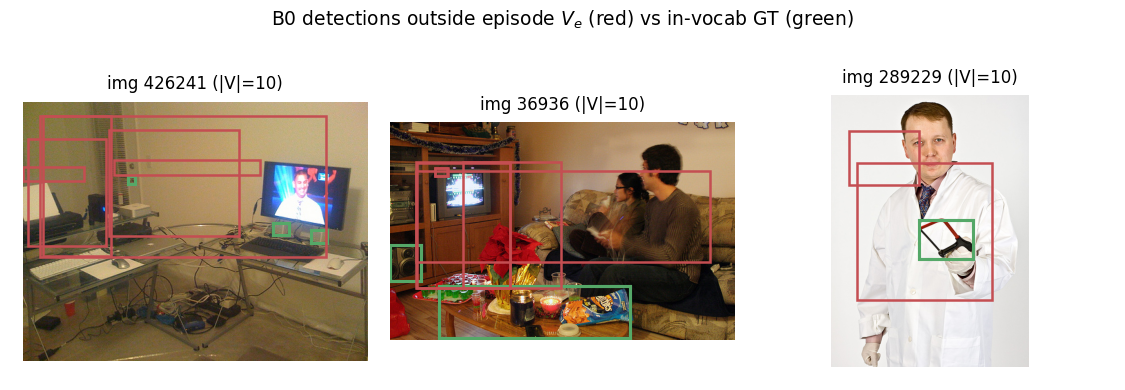
\includegraphics[width=\linewidth]{figures/fig_oov_qualitative.png}
\caption{Qualitative OOV-FP: B0 detections outside episode $V_e$ (cached preds, $|V|{=}10$ dev episode).}
\label{fig:oov_qual}
\end{figure}

\paragraph{Federated AP unchanged.} B0 full minival AP remains \textbf{22.7} (AP$_r$ 16.4)---OVDeploy does not claim benchmark AP gains; it exposes structured deployment behavior invisible to a single AP number.

\paragraph{Seed stability.}
We generate episodes with seeds $\{42,43,44\}$; Tab.~\ref{tab:seed} reports B5/B0 EpisodicAP at $|V|{=}30$, \texttt{noise=none}.
Standard deviation across seeds ($\le 0.4$ AP) is small relative to the B5--B0 gap ($\ge 1.3$ AP), indicating stable deployment trends rather than split artifacts.

\begin{table}[t]
\centering
\small
\begin{tabular}{c cc cc}
\toprule
Seed & B0 & B5 & $\Delta$ & n ep \\
\midrule
42 & 13.4 & 36.0 & +22.6 & 20 \\
43 & 13.9 & 33.6 & +19.7 & 20 \\
44 & 10.9 & 32.3 & +21.3 & 20 \\
\bottomrule
\end{tabular}

\caption{B5 vs B0 EpisodicAP by seed ($|V|{=}30$, noise=none, GPU v2).}
\label{tab:seed}
\end{table}

\paragraph{Metric ablation (v1 vs v2).}
Early episodic AP without greedy IoU matching inflated Oracle scores above 100\% on sparse-GT images.
v2 enforces IoU@0.5 class-consistent matching and caps AP at 100, aligning episodic scores with detection practice.
We recommend v2 for all OVDeploy leaderboard entries.

\paragraph{Episode inventory.}
The public release contains 1,220 episodes: $4$ vocabulary sizes $\times$ $3$ seeds $\times$ $3$ noise modes $\times$ $20$ episodes per configuration on dev, plus train-pool episodes reserved for adapter code only.
Each dev episode references ten minival images and a vocabulary JSON with explicit \texttt{cat\_ids}.
Synonym noise swaps LVIS surface forms; missing-class noise removes one GT class from $V_e$ while leaving annotations intact---stress-testing deployment when user vocabularies are incomplete.

\paragraph{Implementation checklist.}
Each frozen report JSON records \texttt{gpu\_used}, \texttt{metrics\_version}, and UTC \texttt{timestamp}.
Episode JSON, B0 prediction cache, and WSL conda environment \texttt{yoloworld5070} are documented in \texttt{START.md}.
Leaked-image checks (\texttt{REPORT\_leakage\_check.json}) confirm zero overlap between dev and stratified splits.

\section{Discussion}
\label{sec:disc}

\paragraph{Interpreting OOV-FP.}
OOV-FP is intentionally asymmetric: it always measures B0 full-vocabulary behavior against episode $V_e$.
High OOV-FP does not imply low in-vocabulary precision---B5 may score well on $V_e$ while B0 fires on unrelated classes.
For deployment audits, we recommend reporting \textbf{EpisodicAP(B5)} alongside \textbf{OOV-FP(B0)} when the production stack still loads the full prompt table for legacy reasons.

\paragraph{When to use subset prompts.}
B5 requires the application to re-encode prompts when $V_e$ changes; B0 avoids re-encoding but pays in spurious activations.
Fig.~\ref{fig:vcurve}, Fig.~\ref{fig:gap}, and Tab.~\ref{tab:vsweep} show that B5 EpisodicAP gains concentrate at $|V|{\ge}30$, while OOV-FP---always measured on B0---is most severe at small $|V|$.
At $|V|{=}1203$, subset and full vocabularies coincide on LVIS; deployment metrics should always specify $|V|$ and report both EpisodicAP(B5) and OOV-FP(B0) when legacy stacks keep the full prompt table loaded.

\begin{table}[t]
\centering
\small
\setlength{\tabcolsep}{3pt}
\begin{tabular}{@{}p{0.40\linewidth}p{0.20\linewidth}p{0.20\linewidth}@{}}
\toprule
Deployment scenario & Mode & Report \\
\midrule
Legacy full 1203-prompt stack & Audit only (B0) & OOV-FP \\
Known $V$, $|V|{\ge}30$ & Subset encode (B5) & EpiAP + OOV-FP \\
$|V|{\le}10$, incomplete $V$ & Avoid blind subset; B1 upper bound & EpiAP (B1/B5) \\
\bottomrule
\end{tabular}
\caption{\textbf{Deployment guidelines.} OOV-FP diagnoses full-vocabulary errors; B5 subset encoding helps EpisodicAP when $|V|$ is moderate and $V$ is known.}
\label{tab:deploy}
\end{table}

\paragraph{Benchmark positioning.}
OVDeploy is not a new detector; it is an evaluation harness.
We encourage future OVD papers to report at least one episodic row (e.g., $|V|{=}30$ B5 vs B0 EpisodicAP + OOV-FP) alongside federated AP.
Episode JSON and metric code are versioned (\texttt{metrics\_version: v2}) to prevent silent protocol drift.

\paragraph{Multi-backbone check.}
Tab.~\ref{tab:backbone} compares frozen YOLO-World v2-S and OWL-ViT-B/32 on the same OVDeploy episodes ($|V|{\in}\{10,30,100\}$, B0/B5/B1, seed 42, GPU v2).
Both architectures satisfy B5 aggregate EpisodicAP $\ge$ B0 (28 vs 13 on S; 36.1 vs 17.4 on OWL-ViT).
OWL-ViT full-minival B0--B5 on the same held-out 1k (\texttt{REPORT\_4\_full\_owlvit}) mirrors YOLO trends (Tab.~\ref{tab:full_minival}).
At $|V|{=}10$, OOV-FP is 66\% (S) vs 25\% (OWL-ViT), showing that full-vocabulary leakage under small user vocabularies is not unique to one detector family.
Tab.~\ref{tab:backbone_m} adds native \textbf{Microsoft GLIP-T} (\texttt{microsoft/GLIP}, Swin-T \texttt{.pth}; \texttt{REPORT\_6e}) on the same episodes.
B5 aggregate EpisodicAP **34.5** vs B0 **16.9**; B5$\ge$B0 holds while OOV-FP remains high at small $|V|$ (97\% at $|V|{=}10$), matching the YOLO-S / OWL-ViT pattern.
A supplementary \textbf{YOLO-World-M} scale ablation (\texttt{REPORT\_6c}, rebuttal only) gives B5 aggregate **28.7** vs B0 **3.8** with OOV-FP **78\%** at $|V|{=}10$, consistent with the S-scale deployment gap.
Held-out stratified OOV-FP on native GLIP-T (\texttt{REPORT\_4b\_native\_glip}) is reported separately in Tab.~\ref{tab:strat_three}.

\begin{table}[t]
\centering
\small
\begin{tabular}{c l cc cc}
\toprule
$|V|$ & Baseline & \multicolumn{2}{c}{YOLO-World-S} & \multicolumn{2}{c}{OWL-ViT-B/32} \\
 &  & EpiAP & OOV & EpiAP & OOV \\
\midrule
10 & B0-full & 12.7 & 0.664 & 17.5 & 0.251 \\
10 & B1-oracle & 40.9 & 0.664 & 47.3 & 0.251 \\
10 & B5-subset & 20.7 & 0.664 & 29.0 & 0.251 \\
30 & B0-full & 13.4 & 0.553 & 17.0 & 0.221 \\
30 & B1-oracle & 37.9 & 0.553 & 43.1 & 0.221 \\
30 & B5-subset & 36.0 & 0.553 & 42.1 & 0.221 \\
100 & B0-full & 13.4 & 0.480 & 17.6 & 0.171 \\
100 & B1-oracle & 28.2 & 0.480 & 36.6 & 0.171 \\
100 & B5-subset & 26.7 & 0.480 & 37.2 & 0.171 \\
\bottomrule
\end{tabular}

\caption{YOLO-World v2-S vs OWL-ViT-B/32 on OVDeploy dev (GPU v2, \texttt{REPORT\_6}).}
\label{tab:backbone}
\end{table}

\begin{table}[t]
\centering
\scriptsize
\setlength{\tabcolsep}{2pt}
\resizebox{\linewidth}{!}{%
\begin{tabular}{c l cc cc cc}
\toprule
$|V|$ & Baseline & \multicolumn{2}{c}{YOLO-S} & \multicolumn{2}{c}{OWL-ViT} & \multicolumn{2}{c}{GLIP-T} \\
 &  & EpiAP & OOV & EpiAP & OOV & EpiAP & OOV \\
\midrule
10 & B0-full & 12.7 & 0.664 & 17.5 & 0.251 & 16.4 & 0.968 \\
10 & B1-oracle & 40.9 & 0.664 & 47.3 & 0.251 & 54.8 & 0.968 \\
10 & B5-subset & 20.7 & 0.664 & 29.0 & 0.251 & 27.3 & 0.968 \\
30 & B0-full & 13.4 & 0.553 & 17.0 & 0.221 & 17.5 & 0.885 \\
30 & B1-oracle & 37.9 & 0.553 & 43.1 & 0.221 & 47.5 & 0.885 \\
30 & B5-subset & 36.0 & 0.553 & 42.1 & 0.221 & 43.9 & 0.885 \\
100 & B0-full & 13.4 & 0.480 & 17.6 & 0.171 & 16.8 & 0.755 \\
100 & B1-oracle & 28.2 & 0.480 & 36.6 & 0.171 & 32.6 & 0.755 \\
100 & B5-subset & 26.7 & 0.480 & 37.2 & 0.171 & 32.4 & 0.755 \\
\bottomrule
\end{tabular}
%
}
\caption{YOLO-S vs OWL-ViT vs native GLIP-T (\texttt{REPORT\_6e}) on OVDeploy dev (GPU v2).}
\label{tab:backbone_m}
\end{table}

\paragraph{Future extensions.}
Interactive user vocabularies and multilingual prompts are natural extensions.
Episode-level adapters were explored in supplementary code (\texttt{REPORT\_3}); they did not outperform frozen B5 on our GPU dev split and are excluded from main claims.

\section{Limitations and Conclusion}
\label{sec:lim}

OVDeploy episodes sample vocabularies from LVIS statistics rather than live user studies; English-only prompts.
Stratified held-out uses frequency-top-$|V|$ (OOV-FP confirmation); dev episodic uses GT-aligned $V_e$ (B5 deployment reference).
ODinW covers the full ODinW-13 native suite; Pothole/Shellfish remain low ($\sim$0--1 EpisodicAP) and Packages low ($\sim$4) despite synonym prompts---we do not claim cross-domain SOTA.
Grounded OVD main-table cross-check uses native \textbf{Microsoft GLIP-T} (\texttt{microsoft/GLIP}, \texttt{REPORT\_6e}; Tab.~\ref{tab:backbone_m}).
Stratified held-out OOV-FP additionally reports native GLIP-T (\texttt{REPORT\_4b\_native\_glip}, Tab.~\ref{tab:strat_three}) alongside YOLO-S and OWL-ViT.
Native GLIP-T weights (\texttt{GLIPModel/GLIP}) and \texttt{maskrcnn\_benchmark} CUDA ops were rebuilt on WSL (PyTorch 2.11 + CUDA 12.8; \texttt{scripts/wsl\_rebuild\_native\_glip\_cuda.sh}).
OWL-ViT uses locally cached HuggingFace weights; absolute EpisodicAP differs across architectures and should not be compared to federated LVIS AP.
Lightweight episode adapters were explored in supplementary code (\texttt{REPORT\_3}) but are excluded from main baselines (M1 EpisodicAP $\approx$1.6 vs B5 $\approx$25 on dev aggregates).

\textbf{Conclusion.} Federated LVIS AP alone is insufficient for OVD deployment analysis.
OVDeploy provides episodic metrics, 1,220 episodes, and frozen baselines showing that \textbf{OOV-FP} from full-vocabulary inference is severe under small user vocabularies, while subset-prompt deployment (B5) improves aggregate EpisodicAP over B0 under strict greedy matching.

\paragraph{Comparison to federated AP components.}
AP$_r$, AP$_c$, and AP$_f$ on our checkpoint are 16.4, 20.8, and 25.5 respectively---unchanged across OVDeploy baselines because backbone weights are frozen.
Episodic metrics instead answer: ``If I only care about $V_e$ on these images, how often does full-vocabulary inference fire outside $V_e$?'' and ``If I encode only $V_e$, what greedy AP do I obtain?''
These questions are orthogonal to rare-class recall on the full LVIS label space.

\paragraph{Reproducibility artifacts.}
Anonymous code zip: \texttt{release/ovdeploy\_anonymous.zip}; frozen JSON under \texttt{reports/}; one-command WSL pipeline \texttt{scripts/wsl\_rerun\_v2.sh} (full dev matrix, noise eval, stratified 1k, ODinW).

{\small
\bibliographystyle{ieeenat_fullname}
\bibliography{references}
}

\end{document}
